\documentclass[12pt, a4paper]{article}
\usepackage[utf8]{inputenc}
\usepackage[spanish]{babel}
\usepackage{graphicx}
\usepackage{amsmath}
\usepackage{hyperref}

\title{Simulación de compañía de seguros}
\author{Orlando R. de la Torre Leal}
\date{\today}

\begin{document}

\maketitle

\section{Introducción} 
\subsection*{Contexto}
En el proyecto se modela una compañía de seguros de daños donde los titulares de póliza o asegurados realizan reclamaciones
de acuerdo a procesos de Poisson independientes con una tasa en comun $\lambda$ y el costo de cada reclamación tiene distribución
$F$. Nuevos clientes se unen a la compañia acorde a un proceso de Poisson con un ratio $v$. Cada cliente permanece en la compañía
por un tiempo exponencial con tasa $\mu$ antes de darse de baja. Cada asegurado paga a la compañía de seguros una cantidad $c$ por 
unidad de tiempo. 

\subsection*{Objetivos}
Dada una condición inicial de $n_0$ clientes y un capital inicial $a_0 \geq 0$, se busca estimar que a probabilidad de que el 
capital de la compañía nunca sea negativo en el intervalo de tiempo $[0, T]$.

\subsection*{Variables que describen el problema}

Para simular el sistema anterior, definimos las variables y eventos de la siguiente manera:
\\
Variables: 
\begin{itemize}
    \item Variable de tiempo: $t$.
    \item Variable de estado del sistema $(n,a)$, donde $n$ es el numero de asegurados y $a$ es el capital actual de la compañía.
    \item Tasa de llegada de nuevos clientes: $v$
    \item Tasa de abandono por cliente: $\mu$
    \item Tasa de reclamaciones por clientes: $\lambda$
\end{itemize}
Eventos:
\begin{itemize}
    \item LLegada de un nuevo asegurado(titulares)
    \item Pérdida de un asegurado
    \item Reclamación de un asegurado
\end{itemize}
La lista de eventos consiste en un único valor: el tiempo en el que ocurrirá el próximo evento.\\
Notación: $EL = t_E$
Si el estado actual es $(n,a)$ en tiempo $t$, el próximo evento ocurirrá en $t + X$, donde $X$ es una variable
aleatoria exponencial con tasa:
$$ \text{Tasa Total}= v + n\mu + n\lambda$$
Aún así, no importa cuando ocurra el próximo evento, este ocurrirá con una probabilidad:
\begin{itemize}
    \item Nuevo asegurado: $\frac{v}{v+n\mu+n\lambda}$
    \item Pérdida de asegurado: $\frac{n\mu}{v+n\mu+n\lambda}$
    \item Reclamación: $\frac{n\lambda}{v+n\mu+n\lambda}$
\end{itemize}
Tras determinar cuándo ocurre el proximo evento se genera un número aleatorio para identificar
cuál de los tres eventos ocurrió. Luego se actualiza el estado del sistema $(n,a)$ en función del evento seleccionado.

Para un estado $(n,a)$:
\begin{itemize}
    \item $X$: Variable aleatorio exponencial con tasa $v+n\mu+n\lambda$(tiempo hasta el próximo evento).
    \item $J$: Variable aleatoria que representa el tipo de evento.
        \begin{equation}
            J = 
            \begin{cases}
                1 & \text{Nuevo asegurado}, \quad \text{con probabilidad } \dfrac{\nu}{\nu + n\mu + n\lambda}, \\
                2 & \text{Pérdida de asegurado}, \quad \text{con probabilidad } \dfrac{n\mu}{\nu + n\mu + n\lambda}, \\
                3 & \text{Reclamación}, \quad \text{con probabilidad } \dfrac{n\lambda}{\nu + n\mu + n\lambda}
            \end{cases}
        \end{equation}
    \item $Y$: Variable aleatoria con distribución $F$(costo de la reclamación)
    \item $I$: Indicador del éxito financiero:
        \begin{equation}
            I =
            \begin{cases}
                1 & \text{, si el capital es no negativo}, \\
                0 & \text{, en caso contrario}
            \end{cases}
        \end{equation}
\end{itemize}

\section{Detalles de Implementación} 

\subsection*{Inicialización}
Para simular el sistema, inicializamos las variables de la siguiente manera:

\begin{enumerate}
    \item \textbf{Inicialización inicial}:
    \begin{align*}
        t &= 0, \\
        a &= a_0, \\
        n &= n_0
    \end{align*}
    
    \item Generar $X \sim \text{Exponencial}(\nu + n\mu + n\lambda)$(tiempo de espera hasta la siguiente evaluación) e inicializar:
    \begin{align*}
        t_E &= X
    \end{align*}
\end{enumerate}

\subsection*{Actualización}
Para actualizar el sistema, avanzamos al siguiente evento, verificando primero si nos lleva más allá del tiempo $T$:

\begin{enumerate}
    \item \textbf{Caso 1}: Si $t_E > T$:
    \begin{itemize}
        \item Asignar $I = 1$ y finalizar esta ejecución.
    \end{itemize}
    
    \item \textbf{Caso 2}: Si $t_E \leq T$:
    \begin{enumerate}
        \item Reiniciar:
        \begin{align*}
            a &= a + n \cdot c \cdot (t_E)  \\
            t &= t_E \quad 
        \end{align*}
        
        \item Generar $J$:
        \begin{align*}
            J &= 
            \begin{cases}
                1: & n = n + 1 \\
                2: & n = n - 1  \\
                3: & 
                \begin{aligned}
                    &\text{Generar } Y \sim F. \\
                    &\text{Si } Y > a \text{, asignar } I = 0 \text{ y terminar.} \\
                    &\text{En otro caso, } a = a - Y \quad \text{(Pagar reclamación)}
                \end{aligned}
            \end{cases}
        \end{align*}
        
        \item Generar $X \sim \text{Exponencial}(\nu + n\mu + n\lambda)$ y actualizar:
        \begin{align*}
            t_E &= t + X
        \end{align*}
    \end{enumerate}
\end{enumerate}

El paso de actualización se repite continuamente hasta que se completa una ejecución.

\section{Resultados y Experimentos} 
\subsection*{Hallazgos de la simulación}
Para los siguientes valores iniciales:
\begin{itemize}
   \item $v=0.6$ Tasa de nuevos clientes
   \item $\mu=0.3$ Tasa de abandono de clientes
   \item $\lambda = 0.2$ Tasa de reclamaciones de clientes
   \item $c=2.5$ Pago de clientes por unidad de tiempo
   \item $a_0=10$ Capital Inicial
   \item $n_0=5$ Cantidad Inicial de clientes
   \item $T=500$ Tiempo máximo
\end{itemize}
\begin{figure}[h]
    \centering
    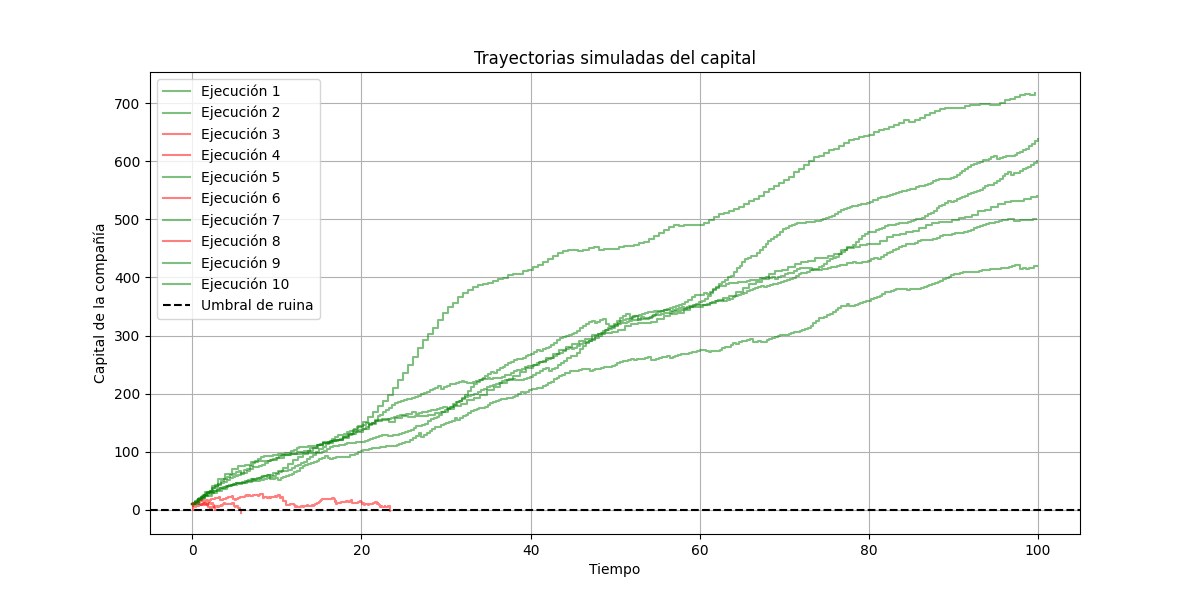
\includegraphics[width=0.8\textwidth]{Figure_1.png}

    \label{fig:1}
\end{figure}
Durante 1000 simulaciones hemos obtenido los siguientes resultados:
\begin{itemize}
    \item Probabilidad de no arruinarse: 0.743\%
    \item Tiempo promedio hasta arruinarse: 75.59 unidades de tiempo
\end{itemize}
\subsection*{Interpretación de los resultados}
El costo actual (c = 2.5) es suficiente para evitar la ruina en al menos el 74.3\% de los casos.
Las reclamaciones grandes (> $a_0$) son la principal causa de ruina temprana (antes de T/2).
\subsection*{Hipótesis extraídas}
\begin{itemize}
    \item El aumento del costo por cliente aumenta la probabilidad de éxito pero no es rentable.
    \item El aumento de la frecuencia de reclamaciones disminuye la probabilidad de exito drámaticamente.
\end{itemize}

\subsection*{Experimentos de validación}
\begin{itemize}
    \item Para la Hipótesis 1 se aumento el costo de 2.5 a 3.0(20\%) y se obtuvo un aumento en la probabilidad de exito de 74.3\% a 77.87\% un mero 3\%, no es rentable. Podría aumentar el descontento ocasionando mas reclamaciones.
    \begin{figure}[h]
        \centering
        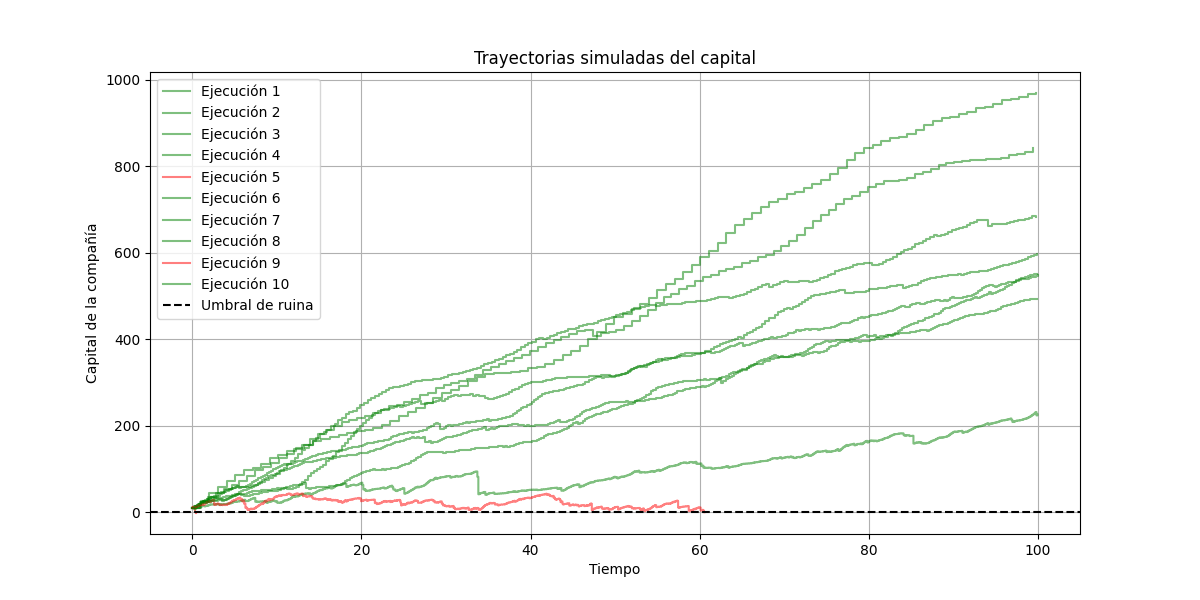
\includegraphics[width=0.8\textwidth]{Figure_2.png}
    
        \label{fig:2}
    \end{figure}
    \item Para la Hipótesis 2 se aumento el ratio de reclamaciones($\lambda = 0.2$ a $\lambda = 0.6$) y disminuyó la probabilidad de éxito hasta un 38.4\% con tiempo estimado de ruina de 41.72u de tiempo
    \begin{figure}[h]
        \centering
        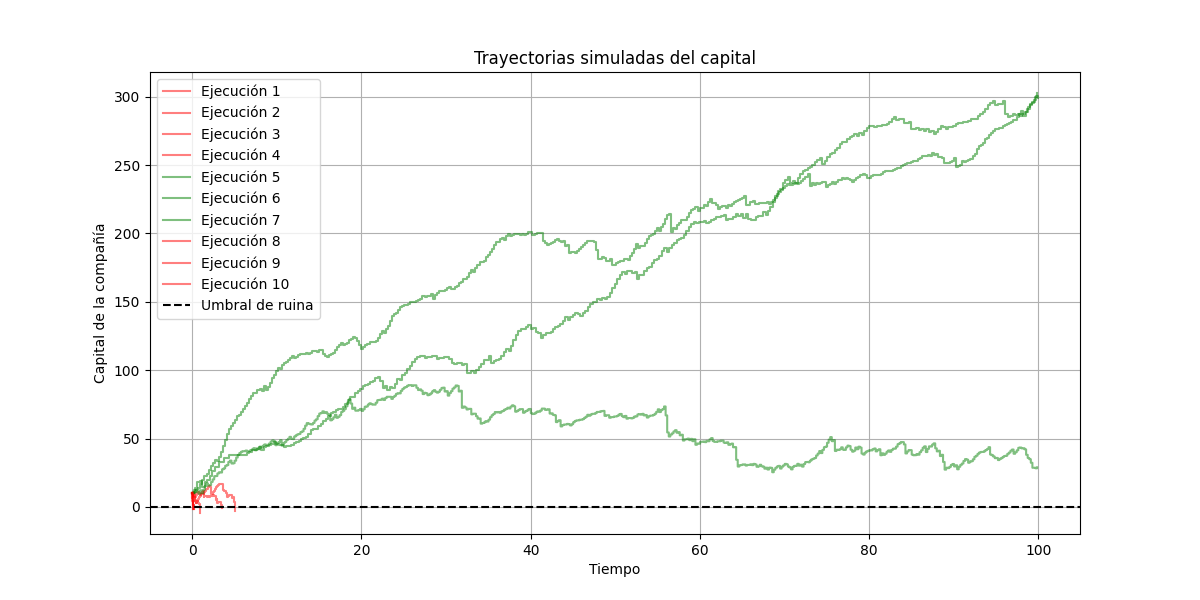
\includegraphics[width=0.8\textwidth]{Figure_3.png}
    
        \label{fig:3}
    \end{figure}
\end{itemize}
\newpage
\subsection*{Análisis de parada}
Si se llega al valor de ruina $a\leq0$ se puede detener la simulación o si se alcanza el final. 

\section{Conclusiones} 
Para maximizar el éxito de una compañía de seguros es importante controlar que la tasa de ingreso de clientes sea mayor que la de retirada($\mu > \lambda$). Y en base a la cantidad de clientes
hay un límite de hasta donde aumentar el precio es rentable para maximizar las ganancias y minimizando las reclamaciones. 

\end{document}